Dynamic graph algorithms support query operations of certain properties on a dynamic graph \cite{graph-italiano99}. Examples of such algorithms include \emph{Dynamic Connectivity (undirected graph)} which tells whether the graph is connected or two given vertices are connected through edges \cite{conn-patrascu04}, \emph{Dynamic Transitive Closure (directed graph)} which tells whether a vertex is reachable from another vertex \cite{conn-demetrescu00}, \emph{Dynamic All Pairs Shortest Path (APSP)} which tells the shortest path and distance between any two vertices \cite{apsp-demetrescu04}, \emph{Dynamic Minimum Spanning Tree (MST)} which determines the value of a property on an MST \cite{mst-henzinger97}, \emph{Dynamic Min Cut} which tells whether two vertices are on the same side on a minimum cut \cite{cut-italiano11}, \emph{Dynamic Planarity} which tells whether the graph is planar (the edges do not cross each other) \cite{planar-galil99}, or \emph{Dynamic k-connectivity} which tells whether the graph is k-connected or whether two given vertices are k-connected (removing fewer than k vertices still maintains connectivity) \cite{conn-liang01} \cite{graph-italiano99}.

Dynamic Centrality, which was first developed in social network analysis \cite{graph-newman18}, is an important category of dynamic graph algorithms which focus on ranking vertices in a graph based on an importance metric \cite{centrality-bonacich87}. It finds applications in identifying super-spreaders of a disease, key infrastructure nodes in the Internet or mobile networks, the most informative websites, influential person(s) in a social network \cite{centrality-borgatti05}, and brain networks \cite{brain-vandenheuvel13} \cite{brain-saberi21}. Importance is conceived as a type of flow across the network, or an involvement in cohesiveness of the network. Eigenvector centrality which measures the influence of a vertex in a graph is a walk based importance metric, and is based on the concept that contributions from important vertices are more important \cite{graph-newman16}. PageRank centrality is a variation of Eigenvector centrality, which measures the importance of a vertex based on its in-bound edges instead of out-bound ones and includes a scaling factor per graph \cite{pr-network20q}.

% Dynamic Centrality, which was first developed in social network analysis \cite{graph-newman18}, is an important category of dynamic graph algorithms which focus on ranking vertices in a graph based on an importance metric \cite{centrality-bonacich87}. It finds applications in identifying super-spreaders of a disease, key infrastructure nodes in the Internet or mobile networks, the most informative websites, influential person(s) in a social network \cite{centrality-borgatti05}, and brain networks \cite{brain-vandenheuvel13} \cite{brain-saberi21}. Importance is conceived as a type of flow across the network, or an involvement in cohesiveness of the network. For a flow-based importance metric, the flow can be conserved (like package delivery) or duplicate-able (like gossip spread); the paths can constrained to geodesics (shortest paths), paths (visit vertices once), trails (visit edges once) or walks (no limit); walks can be made from a given vertices (radial), or through a given vertex (medial); and the counting can capture walk volume (total number of walks), or walk length (distance from given vertex to remaining vertices) \cite{centrality-borgatti05} \cite{centrality-borgatti06}.

% A centrality which is optimal for one application is often sub-optimal for another application, and is the reason why we need so many different centralities \cite{politics-krackhardt90}. It should also be noted that centrality algorithms focus obtaining the most important vertices, and the rankings do not necessarily generalize to the remaining vertices \cite{centrality-lawyer15} \cite{epidemic-dasilva12} \cite{epidemic-bauer12} \cite{epidemic-sikic13}. The popular varieties of centralities include Degree centrality which is defined as the number of edges pointing to a vertex, Closeness centrality which inverse average shortest path length between a given vertex and all other vertices in the graph \cite{centrality-bavelas50} \cite{centrality-sabidussi66}, Betweenness centrality which measures the number of times a vertex acts as a bridge along the shortest path between any two vertices \cite{centrality-freeman77}, Eigenvector centrality which measures the influence of a vertex in a graph and is based on the concept that contributions from important vertices are more important \cite{graph-newman16}, Katz centrality (a variation of Eigenvector centrality) which measures the number of vertices that can be connected through a path while penalizing contributions from distant vertices \cite{centrality-katz53}, PageRank centrality (another variation of Eigenvector centrality) which measures the importance of a vertex based on its in-bound edges instead of out-bound ones (in Eigenvector, Katz centrality) and includes a scaling factor per graph \cite{pr-network20q}, Percolation centrality which measures the importance of a vertex based on the percolation on a state from one vertex to another in a time-dependent manner \cite{centrality-piraveenan13}, and Cross-clique centrality which measures the connectivity of a vertex to different cliques (a subgraph where every pair of vertices are adjacent) \cite{centrality-everett98} \cite{social-faghani13}.

We focus on studying algorithms for ranking vertices in a graph using the PageRank algorithm, detecting communities using the Louvain algorithm, and maintaining graph data structures on the CPU, GPU, or other computing devices. Note that there are several alternative approaches for ranking vertices in a graph, or identifying communities in a graph, but we focus on the most commonly used algorithm for each problem.




\section{PageRank Algorithm}

The \textbf{PageRank algorithm} is a technique used to sort vertices of a graph (or web pages) by importance. It is quite popularly the algorithm published by the founders of Google. Other link analysis algorithms include \textbf{HITS} \cite{hits-chien14}, \textbf{TrustRank} \cite{pr-gyongyi04}, and \textbf{HummingBird} \cite{pr-patil21}. Such link-analysis algorithms are also used for word sense \textbf{disambiguation} in lexical semantics, urban planning \cite{urban-zhang18}, ranking streets by traffic \cite{traffic-kim15}, identifying \textbf{communities} \cite{pr-kloumann17}, measuring their \textbf{impact} on the web, maximizing influence \cite{influence-zhang15}, providing \textbf{recommendations} \cite{recommend-chaudhari17}, analysing neural/protein networks, determining species \textbf{essential} for health of the environment, or even quantifying the \textbf{scientific impact} of researchers \cite{pr-senanayake15}.

In order to understand the PageRank algorithm, consider the \textbf{random surfer model} on a graph with several vertices and interconnecting edges. The surfer (such as you) initially visits a vertex at random. He then follows one of the edges leading to another vertex. After following some edges, the surfer would eventually decide to visit another vertex (at random). The probability of the random surfer being on a certain vertex is what the PageRank algorithm returns. This probability (or importance) of a vertex depends upon the importance of vertices pointing to it. This definition of PageRank is recursive, and takes the form of an \textbf{eigen-value problem}. Solving for PageRank thus requires multiple iterations of computation, which is known as the \textbf{power-iteration method}. Each computation is essentially a \textbf{(sparse) matrix multiplication}. A damping factor (of 0.85) is used to counter the effect of \textbf{spider-traps} (like self-loops), which can otherwise suck up all importance. \textbf{Dead-ends} (vertices with no out-links) are countered by effectively linking it to all vertices of the graph, which otherwise would leak out importance \cite{pr-leskovec19}. See Figure \ref{fig:about-pagerank} for example. The procedure to obtain such ranks is shown in Algorithm \ref{alg:pr-static}.
% (\textbf{Markov chain}) (making Markov matrix column stochastic)
% In order to understand the PageRank algorithm, consider this \textbf{random (web) surfer model}. Each web page is modelled as a vertex, and each hyperlink as an edge. The surfer (such as you) initially visits a web page at random. He then follows one of the links on the page, leading to another web page. After following some links, the surfer would eventually decide to visit another web page (at random). The probability of the random surfer being on a certain page is what the PageRank algorithm returns. This probability (or importance) of a web page depends upon the importance of web pages pointing to it (\textbf{Markov chain}). This definition of PageRank is recursive, and takes the form of an \textbf{eigen-value problem}. Solving for PageRank thus requires multiple iterations of computation, which is known as the \textbf{power-iteration method}. Each computation is essentially a \textbf{(sparse) matrix multiplication}. A damping factor (of 0.85) is used to counter the effect of \textbf{spider-traps} (like self-loops), which can otherwise suck up all importance. \textbf{Dead-ends} (web pages with no out-links) are countered by effectively linking it to all vertices of the graph (making Markov matrix column stochastic), which otherwise would leak out importance \cite{pr-leskovec19}. See \ref{fig:about-pagerank} for example. The procedure to obtain such ranks is shown in algorithm \ref{alg:pr-static}.

\begin{figure}[hbtp]
  \centering
  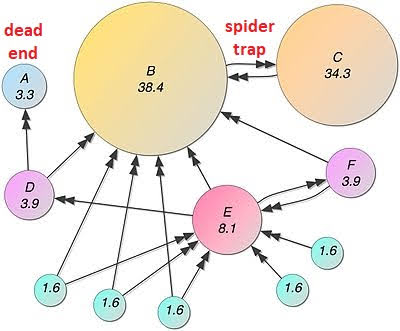
\includegraphics[width=0.60\textwidth]{out/about-pagerank.jpg}
  \caption{Example of web pages with hyperlinks and respective PageRanks \cite{pr-jardine07}.}
  \label{fig:about-pagerank}
\end{figure}

\vspace{2em}
\begin{algorithm}[!hbtp]
\caption{Algorithm for computing \emph{static PageRank} (static Monolithic). Here, $G$ is the current snapshot of the graph.}
\label{alg:pr-static}
\begin{algorithmic}
% \Require{$G$: Graph (V, E)}
\Function{staticPR}{$\vars{G}$}
\State $V \gets G.vertices$
\State $n \gets G.order$
\ForAll{$u \in V$} \textbf{in parallel}
  \State $prev_u = 1/n$
\EndFor
\Return{$\textsc{monolithicLoop}(G, [V], prev)$}
\EndFunction

\Statex

\Function{monolithicLoop}{$\vars{G}, \vars{SCCs}, \vars{prev}$}
  \State $MAX\_ITERS \gets 500$
  \State $\tau \gets TOLERANCE = 10^{-6}$
  \ForAll{$l \in range(0, MAX\_ITERS)$}
    \State $pr \gets \textsc{calculateRanks}(G, SCCs, prev)$
    \If{$l\infty{}Norm(prev, pr) < \tau$}
        \State $\textrm{break}$
    \EndIf
    \State $prev \gets pr$
  \EndFor
  \Return{$pr$}
\EndFunction

\Statex

\Function{calculateRanks}{$\vars{G}, \vars{SCCs}, \vars{prev}$}:
  \State $d \gets DAMPING = 0.15$
  \State $n \gets G.order$
  \State $outdeg \gets G.outDegrees$
  \ForAll{$SCC \in SCCs$} \textbf{in parallel}
    \ForAll{$v \in SCC$} \textbf{in parallel}
      \State $pr_v = d/n + (1 - d) * \Sigma _{u \in in(v)} \frac{prev_u}{outdeg_u}$
    \EndFor
  \EndFor
  \Return{$pr$}
\EndFunction
\end{algorithmic}
\end{algorithm}
\vspace{1em}


% Note that as originally conceived, the PageRank model does not factor a web browser's \textbf{back button} into a surfer's hyperlinking possibilities. Surfers in one class, if teleporting, may be much more likely to jump to pages about sports, while surfers in another class may be much more likely to jump to pages pertaining to news and current events. Such differing teleportation tendencies can be captured in two different \textbf{personalization vectors}. However, it makes the once query-independent, user independent PageRankings, user-dependent and more calculation-laden. Nevertheless, it seems this little personalization vector has had more significant side effects. This personalization vector, along with a \textbf{non-uniform/weighted} version of PageRank \cite{pr-dubey16} can help control spamming done by the so-called link farms \cite{pr-deeper01}.

PageRank algorithms almost always take the following \textbf{parameters}: damping, tolerance, and maximum number of iterations allowed. Here, \textbf{tolerance} defines the error between the previous and the current iterations. Though this is usually $L_1$-norm, $L_2$ and $L_\infty$-norm are also used sometimes. Both damping and tolerance control the rate of convergence of the algorithm. The choice of tolerance function also affects the rate of convergence. However, adjusting \textbf{damping} can give completely different PageRank values. Since the ordering of vertices is important, and not the exact values, it can usually be a good idea to choose a larger tolerance value.

Techniques to optimize the PageRank algorithm usually fall in two categories. One is to try \textbf{reducing the work per iteration}, and the other is to try \textbf{reducing the number of iterations}. Often, these goals are at odds against each other. The \textbf{adapting PageRank technique} "locks" vertices which have converged, and saves iteration time by skipping their computation \cite{pr-deeper01}. Identical nodes, which have the same in-links, can be removed to reduce duplicate computations and thus reduce iteration time. Road networks often have chains which can be short-circuited before PageRank computation to improve performance. Final ranks of chain nodes can be easily calculated. This reduces both the iteration time, and the number of iterations. If a graph has no dangling nodes, PageRank of each strongly connected component can be computed in topological order. This helps reduce the iteration time, number of iterations, and also enable concurrency in PageRank computation. The combination of all of the above methods is the \textbf{STIC-D algorithm} (see Figure \ref{fig:about-pagerank-sticd}) \cite{pr-sticd16}. A somewhat similar aggregation algorithm is \textbf{BlockRank} which computes the PageRank of hosts, local PageRank of pages within hosts independently, and aggregates them with weights for the final rank vector. The ranks of vertices for the entire graph can be found efficiently by computing the sub-PageRank of each connected component, and then using the sub-PageRanks together to form the global PageRank (Avrachenkov et. al. \cite{pr-avrachenkov04}). These methods exploit the inherent reducibility in the graph. The \textbf{Jacobi method} can also be used to compute the PageRank vector (Bianchini et. al. \cite{pr-bianchini05}) \cite{pr-deeper01}. \textbf{Monte Carlo} based PageRank methods consider several random walks on the input graph to get approximate PageRanks. Its optimizations for distributed PageRank computation (specially for undirected graphs) \cite{compute-frey13}, map-reduce algorithm for personalized PageRank \cite{pr-bahmani11}, and reordering strategy (to reduce space and compute complexity on GPU) for local PageRank \cite{pr-lai17} are present.

\begin{figure*}[hbtp]
  \centering
  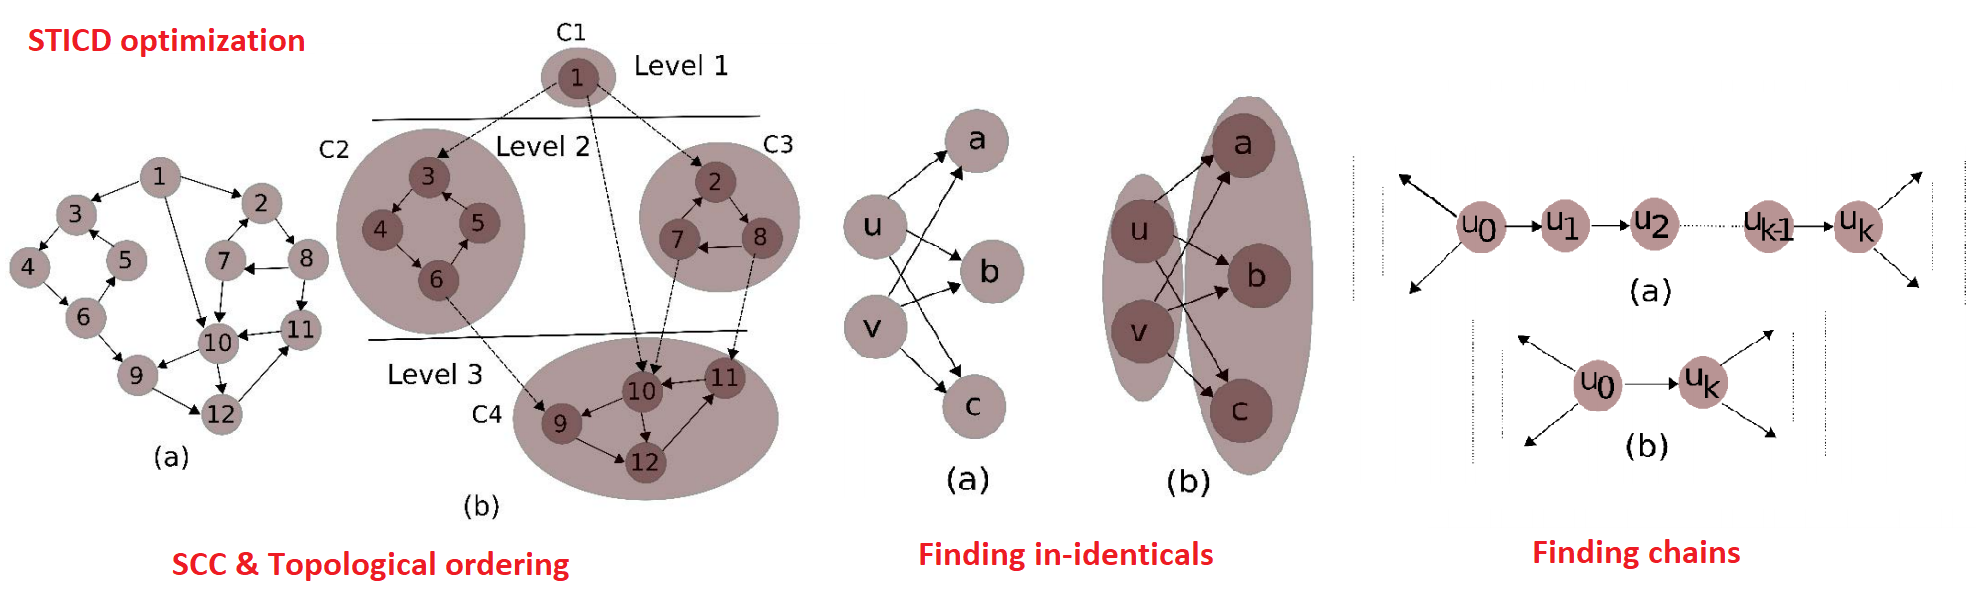
\includegraphics[width=0.98\textwidth]{out/about-pagerank-sticd.png}
  \caption{STIC-D: Algorithmic optimizations for PageRank \cite{pr-sticd16}.}
  \label{fig:about-pagerank-sticd}
\end{figure*}



% The time per iteration can be reduced further by taking note of the fact that the traditional algorithm is \textbf{not computationally bound} and \textbf{generates fine granularity random accesses} (it exhibits irregular parallelism). This causes poor memory bandwidth and compute utilization, and the extent of this is quite dependent upon the graph structure \cite{compute-hunold15} \cite{pr-lakhotia18}. \textit{Four strategies for neighbour iteration} were attempted, to help reason about the \textit{expected impact of a graph's structure} on the performance of each strategy \cite{compute-hunold15}. CPUs/GPUs are generally designed optimized to \textbf{load memory} in blocks (cache-lines in CPUs, coalesced memory reads in GPUs), and not for fine-grained accesses. Being able to adjust this behaviour depending upon application (PageRank) can lead to performance improvements. Techniques like \textit{prefetching to SRAM, using a high-performance shuffle network} \cite{graph-wang15}, \textit{indirect memory prefetcher (of the form $A[B[i]]$), partial cache line accessing mechanisms} \cite{memory-yu15}, \textit{adjusting data layout} \cite{pr-lakhotia18} \textit{(for sequential DRAM access} \cite{pr-zhou15} \textit{), and branch avoidance mechanisms (with partitioning)} \cite{pr-lakhotia18} are used. Large graphs can be \textbf{partitioned }or decomposed into subgraphs to help reduce cross-partition data access that helps both in distributed, as well as shared memory systems (by reducing random accesses). Techniques like \textit{chunk partitioning} \cite{pr-rungsawang12}, \textit{cache/propagation blocking} \cite{pr-beamer17}, \textit{partition-centric processing with gather-apply-scatter model} \cite{pr-lakhotia18}, \textit{edge-centric scatter-gather with non-overlapping vertex-set} \cite{pr-zhou17}, \textit{exploiting node-score sparsity} \cite{pr-li21}, and even \textit{personalized PageRank based partitioning} \cite{pr-mazaheri19} have been used. Graph/subgraph \textbf{compression} can also help reduce memory bottlenecks \cite{pr-rungsawang12} \cite{pr-guoqiang20}, and enable processing of larger graphs in memory. A number of techniques can be used to compress adjacency lists, such as, \textit{delta encoding of edge/neighbour ids} \cite{graph-bharat98}, and \textit{referring sets of edges in edge lists} \cite{graph-adler01} \cite{graph-raghavan03} (hard to find reference vertices though) \cite{pr-deeper01}. Since the rank vector (possibly even including certain additional page-importance estimates) must reside entirely in main memory, a few compression techniques have been attempted. These include \textit{lossy encoding schemes based on scalar quantization} seeking to minimize the distortion of search-result rankings \cite{pr-haveliwala02} \cite{pr-deeper01}, and using \textit{custom half-precision floating-point formats} \cite{pr-molahosseini20}.

As new software/hardware \textbf{platforms} appear on the horizon, researchers have been eager to test the performance of PageRank on the hardware. This is because each platform offers its own unique architecture and engineering choices, and also because PageRank often serves as a good benchmark for the capability of the platform to handle various other graph algorithms. Attempts have been made on distributed frameworks like \textit{Hadoop} \cite{pr-abdullah10}, and even \textit{RDBMS} \cite{compute-barolli21}. A number of implementations have been done on \textit{standard multicores} \cite{compute-barolli21}, \textit{Cell BE} \cite{compute-buehrer08} \cite{pr-zhou17}, \textit{AMD GPUs} \cite{pr-wu10}, \textit{NVIDIA/CUDA GPUs} \cite{pr-bisson16} \cite{pr-zhou17} \cite{graph-seo15}, \textit{GPU clusters} \cite{pr-rungsawang12}, \textit{FPGAs} \cite{pr-mughrabi21} \cite{graph-wang15} \cite{pr-guoqiang20}, \textit{CPU-FPGA hybrids} \cite{pr-hassan21} \cite{pr-usta21} \cite{pr-li21}, and even on SpMV \textit{ASICs} \cite{pr-sadi18}.

PageRank algorithm is a \textbf{live algorithm} which means that an ongoing computation can be paused during graph update, and simply be resumed afterwards (instead of restarting it). The first \textbf{updating} paper by Chien et al. \cite{pr-chien01} identifies a tiny region of the graph near the changed vertices/edges and model the remainder of the graph as a single vertex in a new, much smaller graph. PageRanks are computed for the small graph and then transferred to the original graph \cite{pr-deeper01}. A common technique used for dynamic PageRank algorithm, given a small change to the input graph, is to find the affected region in the preprocessing step with breadth-first search (BFS) or depth-first search (DFS) traversal from the vertices connecting the edges that were inserted or deleted \cite{pr-desikan05} \cite{pr-giri20}.




\section{Community Detection}

Communities are a groups of nodes in a network that correspond to functional units of a system (meta-nodes) \cite{com-chatterjee19}. \textbf{Community detection} schemes can be classified into three basic approaches: bottom-up, top-down, and data-structure based. The bottom-up approach includes the majority of algorithms, so further classification is possible \cite{com-souravlas21}. They can also be classified into three groups, namely: divisive, agglomerative, and multi-level (usually better) \cite{com-zarayeneh21}. The Louvain method for community detection extracts communities from large networks, and created by Blondel et al. \cite{com-blondel08} from the University of Louvain. It is a greedy optimization method with an average time complexity of $\Theta (n \log n)$, with $n$ being the total number of nodes in the network \cite{com-lancichinetti09}.

The idea behind this method is the optimization of modularity iteratively. \textbf{Modularity} is a metric that lies between -0.5 (non-modular communities) and 1 (fully modular communities) for any network, and measures the relative density of links inside communities in contrast to those outside communities. Optimizing modularity theoretically results in the best possible clustering of the nodes. However, as going through each possible clustering of the nodes is impractical, heuristic algorithms such a the Louvain method are used \cite{com-lancichinetti09}.

Louvain algorithm obtains hierarchical communities as a dendrogram through modularity optimization. Given an undirected weighted graph, all vertices are first considered to be their own communities. In the first phase, each vertex greedily decides to move to the community of one of its neighbors which gives the greatest increase in modularity. If moving to no neighbor's community leads to an increase in modularity, the vertex chooses to stay with its own community. This is done sequentially for all the vertices, as per the original algorithm. If the total change in modularity is more than a certain threshold, this phase is repeated. Once this \textbf{local moving phase} is complete, all vertices have formed their first hierarchy of communities. The next phase is called the \textbf{aggregation phase}, where all the vertices belonging to a community are collapsed into a single super-vertex, such that edges between communities are represented as edges between respective super-vertices (edge weights are combined), and edges within each community are represented as self-loops in respective super-vertices (again, edge weights are combined). Together, the local moving and the aggregation phases constitute a stage. This super-vertex graph is then used as input for the next stage. This process continues until the increase in modularity is below a certain threshold. As a result from each stage, we have a hierarchy of community memberships for each vertex as a dendrogram \cite{com-leskovec21}.

Approaches to perform the Louvain algorithm can be divided into \textbf{coarse-grained and fine-grained}. Coarse-grained approaches process a set of vertices in parallel, while fine-grained approaches process all vertices in parallel. A coarse-grained hybrid-GPU algorithm using multi GPUs has been implemented by Cheong et al. \cite{com-cheong13} which grabbed my attention. In addition, their algorithm does not use hashing for the local moving phase, but instead sorts each neighbor list based on the community id of each vertex \cite{com-naim17}.

It should be noted though that community detection methods such as the Louvain that rely on modularity maximization are known to suffer from \textbf{resolution limit problem}. This prevents identification of communities of certain sizes \cite{com-ghosh19}. The \textbf{other major community detection / clustering methods} include: Girvan-Newman or Edge betweenness, the Walktrap, the Louvain, and the CNM \cite{com-drakopoulos18}.

The Louvain algorithm has been implemented using \textbf{OpenMP} \cite{com-bhowmick13} \cite{com-lu15} \cite{com-sattar19}. Heuristics are used to break the sequential barrier \cite{com-lu15}, and load balancing is used to overcome the performance bottleneck \cite{com-sattar19}. It has also been implemented on \textbf{multicore platforms} \cite{com-fazlali17} \cite{com-gheibi20} \cite{part-hossain21} with adaptive parallel thread assignment \cite{com-fazlali17}, cache efficient implementation \cite{com-gheibi20}, and scatter instructions on 512-bit vectors (AVX-512) \cite{part-hossain21}. Platforms used range from an AMD multicore system \cite{com-fazlali17}, and Intel’s Knight's Landing, Haswell \cite{com-gheibi20}, SkylakeX, and Cascade Lake \cite{part-hossain21}. On \textbf{distributed systems} \cite{com-zeng18} \cite{com-ghosh19} \cite{com-sattar19}, the approaches use heuristics for coordinating community constitution in a distributed environment \cite{com-zeng18}, edge-balanced graph distribution for distributed memory implementation \cite{com-ghosh19}, and parallel load-balancing (OpenMPI) \cite{com-sattar19}. Platforms used range from Blue Gene/Q nodes \cite{com-zeng18}, P7-IH nodes \cite{com-zeng18}, and the ALCF Theta supercomputer \cite{com-ghosh19}.

Louvain algorithm based community detection has been implemented on single \cite{com-forster16} \cite{com-naim17} \cite{com-cheong13} \cite{com-mohammadi20} \cite{com-fontolan20} \cite{com-ghoshal19} \cite{com-sattar20} and multi-\textbf{GPUs} \cite{com-cheong13}. These methods use shared memory on the GPU, and use an optimal number of threads for computing modularity \cite{com-mohammadi20} \cite{com-naim17}. Sort-reduce paradigm with pruning on the input data \cite{com-fontolan20}, or hash-based approaches have been used \cite{com-naim17} \cite{com-fontolan20}. Hybrid CPU-GPU systems have been developed \cite{compute-hunold15} \cite{com-bhowmik19} \cite{com-souravlas20} \cite{com-alayyoub19} that use fine-grained parallelism on the GPU \cite{compute-hunold15}, and identify and move doubtful vertices between the devices \cite{com-bhowmik19}.
% Several parallelization heuristics for the Louvain algorithm have been implemented in Grappolo software library \cite{com-halappanavar17}. % Four major community detection algorithms have been implemented in Neo4j: Girvan-Newman or Edge betweenness, the Walktrap, the Louvain, and the CNM \cite{com-drakopoulos18}.

Some \textbf{improvements on the Louvain algorithm} include using a suitable heuristic based partitioning \cite{com-zeng15}, dealing with ghost vertices between graph partitions \cite{com-zeng15},  restricting the internal search rules \cite{com-ryu16}, and early pruning of the non-promising candidates \cite{com-ryu16}. Other interesting approaches include the use of MapReduce in a BigData batch processing framework \cite{com-zeitz17}. For cases where the dynamic graph can undergo abrupt changes, a change-aware model has been developed that detects the type of changes using least information \cite{com-samie17}.

% Community detection based on the \textbf{Infomap algorithm} \cite{com-zeng19} \cite{com-zeng18} \cite{com-faysal19} has been carried out by extending an existing asynchronous distributed framework while ensuring balanced workload and communication \cite{com-zeng19} \cite{com-faysal19}, and using a new heuristic to carefully coordinate the community constitution from the vertices to achieve convergence \cite{com-zeng18}. The Infomap algorithm finds communities by trying to minimize a cost function. The objsectionective is to try to minimize the cost of communicating across a random path between a sender and a receiver by trying to minimize the size of the message \cite{infomap-rosvall09} \cite{com-rita20}.

% Community detection has also been performed with the use of the \textbf{Label propagation algorithm}. It has pros with respect to its execution time, and the lack of additional information required about network structure. It however produces an aggregate of acceptable solutions, but not a unique one \cite{com-newman04}. At the start of the algorithm, each vertex is initialized with a unique label. These labels are then diffused across the graph. Well connected groups reach a common label quickly and continue to expand outwards until it is impossible to do so \cite{com-raghavan07}. A direction optimizing label propagation algorithm which utilizes frontiers, parameter controlled vertex processing order, and alternates between label push and pull operations, has been observed to reduce the number of edges visited and improve the quality of solution \cite{com-liu20}. GPU accelerated parallel label propagation implementation is also available that is able to deal with large-scale datasets that do not fit into GPU memory \cite{com-kozawa17}.

% Community detection based on the use of \textbf{genetic algorithm} \cite{com-taufan20} \cite{com-ghoshal19} \cite{com-lu20} has been achieved based on on diameter of the communities \cite{com-ghoshal19}, using multi-objective optimization with modularity index and a restricted diameter size of clusters \cite{com-lu20}, and adding a cleanup feature in process \cite{com-taufan20}.

% Other \textbf{alternative strategies to the Louvain algorithm} for community detection include combining multilevel graph contraction with core clustering algorithms \cite{com-ruan15}, using a divide and agglomerate algorithm \cite{com-liu19}, using the diameter of a community as a heuristic \cite{com-ghoshal17}, using the CEIL scoring function \cite{com-jain17}, using a game-theoretic approach based on modified modularity along with a new fitness function \cite{com-chopade17}, using fuzzy C-means and K-means algorithm \cite{com-alayyoub19}, using semi-supervised learning with Graph Convolutional Network (GCN) while applying mini-batch gradient descent for larger datasets \cite{com-sattar20}, and the Leiden algorithm which guarantees well connected communities through additional refinement steps in both the local-moving and agglomeration phase \cite{com-traag19}. Communities obtained with differing approaches can be compared with the following \textbf{metrics}: Modularity score \cite{com-ghoshal19}, Normalized Mutual Information (NMI) index \cite{com-jain17} \cite{com-chopade17}, and Jaccard Index \cite{com-jain17}.

% We now discuss a set of related papers in detail. The first paper is on “\textbf{Parallel Heuristics for Scalable Community Detection}” by Lu et al. \cite{com-lu15}. Here, the authors describe the issues with trying to parallelize: possibility of negative gain, community swapping, stuck in local optima. Heuristics like minimum labeling, vertex coloring, and vertex following. Implementation is in OpenMP C++ and they used STL map for communities each vertex is connected to (i was trying this with pre-counting instead which could be faster). They compare using modularity scores mostly. Specificity, Sensitivity, Overlap quality, and Rand index are difficult to calculate for large graphs (based on true positive, false positive, FN, TN). Modularity gain thresholds 10-2, 10-4. Comparison is also with label propagation based parallelization (PLM). There is also another community detection method called Clauset Newman Moore (CNM) which is agglomerative (cluster hierarchies tend to be more meaningful) \cite{com-lu15}.

% The second paper is on “\textbf{From Louvain to Leiden: guaranteeing well connected communities}” by Traag et al. \cite{com-traag19}. They show that some communities produced by the Louvain method are badly connected, and some even disconnected (and why this is not good). The Louvain method relies on modularity score, which has resolution issues (cant handle too small communities, solution CPM score). They add a refinement step and a better (random) local move approach. The restructuring phase is also with a refinement step. They also proved in the supplementary section why it's better \cite{com-traag19}.

% The third paper is on “\textbf{Community detection on the GPU}” by Naim et al. \cite{com-naim17}. The implementation in this paper uses the fine-grained approach such that each edge (not in all cases) is assigned a thread. Vertices are ordered by degree and partitioned by degree into buckets. For the smaller buckets, each edge is assigned a thread. For medium-degree buckets, multiple edges (in interleaved fashion) are assigned to each thread. For larger buckets, multiple vertices may be assigned to each thread block. Open addressing double-hashing is used for obtaining the total weight of communities linked to each vertex. For smaller buckets shared memory is used for storing the hash table, but for larger buckets, global memory is used. Due to global memory limits, execution of some large-degree vertices need to be performed sequentially. The size of a hash table is a precomputed prime number such that its size is at least 1.5 times the degree of the vertex. Note that community ids have to be stored as well. The algorithm implemented in this paper is lock free, and uses only atomic add and compare-and-swap (CAS) operations. Only moves of vertices from higher community id to lower community id are allowed to avoid race conditions. If two possible moves have the same delta-modularity, then the move to lower community id is chosen. Note that as the moving of vertices is performed in parallel, only community memberships of vertices from the previous iteration can be used (relaxed approach), unlike the sequential approach. Aggregation of communities into super-vertices in a new graph CSR is also performed on the GPU with similar thread management and hash tables \cite{com-naim17}. In addition, the authors employ the idea of using higher threshold for modularity gain in the initial rounds. Speedup is observed to be critically dependent upon threshold value. The relaxed strategy of local moving used here also leads to significantly reduced number of phases in certain cases, though this is offset by the algorithm spending more time in each iteration \cite{com-naim17}.

% The fourth paper is on “\textbf{Delta-Screening: A Fast and Efficient Technique to Update Communities in Dynamic Graphs}” by Zarayeneh et. al \cite{com-zarayeneh21}. In this paper, heuristics for skipping out most likely unaffected vertices for a modularity-based community detection method like Louvain and SLM (Smart Local Moving) is given. All edge batches are undirected, and sorted by source vertex id. For edge additions, source vertex i, highest modularity changing edge vertex j*, i's neighbors, and j*'s community are marked as affected. For edge deletions, where i and j must be in the same community, i, j, i's neighbors, and i's community are marked as affected. Performance is compared with static, dynamic baseline (incremental), and this method (both Louvain and SLM). Comparison is also done with "DynaMo" and "Batch" community detection methods \cite{com-zarayeneh21}.
